%
% Chapter 7.5
%

\section*{7.5 Techniques of Integration}

\subsection*{Integration Formulas (without constants of integration)}

\[ \int{x^n dx} = \frac{x^{n+1}}{n+1} \quad (n \neq -1) \]
\[ \int{\frac{1}{x}dx} = \ln{|x|} \]
\[ \int{e^xdx} = e^x \]
\[ \int{b^xdx} = \frac{b^x}{\ln{b}} \]
\[ \int{\sin{x}dx} = - \cos{x} \]
\[ \int{\cos{x}dx} = \sin{x} \]
\[ \int{\sec^2{x}dx} = \tan{x} \]
\[ \int{\csc^2{x}dx = - \cot{x}} \]
\[ \int{\sec{x}\tan{x}dx} = sec{x} \]
\[ \int{\csc{x}\cot{x}dx} = - \csc{x} \]
\[ \int{\sec{x}dx} = \ln{| \sec{x} + \tan{x} |} \]
\[ \int{\csc{x}dx} = \ln{|\csc{x} - \cot{x}|} \]
\[ \int{\tan{x}dx} = \ln{|\sec{x}|} \]
\[ \int{\cot{x}dx} = \ln{|\sin{x}|} \]
\[ \int{\sinh{x}dx} = \cosh{x} \]
\[ \int{\cosh{x}} = \sinh{x} \]
\[ \int{\frac{dx}{x^2 + a^2}} = \frac{1}{a} \tan^{-1} \Big( \frac{x}{a} \Big) \]
\[ \int{\frac{dx}{\sqrt{a^2 - x^2}}} = \sin^{-1} \Big( \frac{x}{a} \Big) \quad \text{when} \quad a > 0 \]
\[ \int{\frac{dx}{x^2 - a^2}} = \frac{1}{2a} \ln{ \Big| \frac{x-a}{x+a} \Big| } \]
\[ \int{\frac{dx}{\sqrt{x^2 \pm a^2}}} = \ln{| x + \sqrt{x^2 \pm a^2} |} \]

\subsection*{Strategies for Integration}

\tikzstyle{item} = [rectangle, minimum height=0.8cm,text centered, draw=black, fill=gray!30]
\tikzstyle{arrow} = [thick,->,>=stealth]

\begin{center}
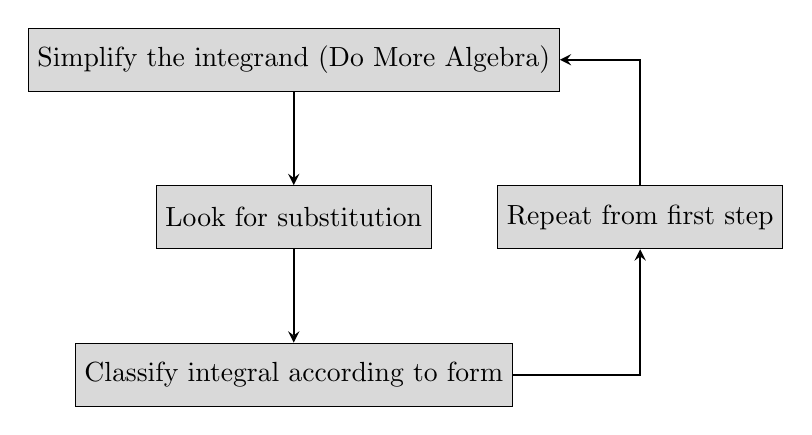
\begin{tikzpicture}[node distance=2cm]
\node (step1) [item] {Simplify the integrand (Do More Algebra)};
\node (step2) [item, below of=step1] {Look for substitution};
\node (step3) [item, below of=step2] {Classify integral according to form};
\node (step4) [item, right of=step2, xshift=2.4cm] {Repeat from first step};

\draw [arrow] (step1) -- (step2);
\draw [arrow] (step2) -- (step3);
\draw [arrow] (step3) -| (step4);
\draw [arrow] (step4) |- (step1);
\end{tikzpicture}
\end{center}
